\documentclass{beamer}
\usepackage[utf8]{inputenc}
%\usepackage[czech, english]{babel}
\usepackage{czech}
\usetheme{Warsaw}
\title[Demonstrační aplikace pro podporu kurzu neuronových sítí]{Demonstrační aplikace pro podporu kurzu neuronových sítí}
\author{Adam Činčura}
\institute{ČVUT - FEL}
\date{28. 6. 2011}
\defbeamertemplate*{footline}{shadow theme}
{%
  \leavevmode%
  \hbox{\begin{beamercolorbox}[wd=.47\paperwidth,ht=2.5ex,dp=1.125ex,leftskip=.3cm plus1fil,rightskip=.3cm]{author in head/foot}%
    \usebeamerfont{author in head/foot}\insertshortauthor
  \end{beamercolorbox}%
  \begin{beamercolorbox}[wd=.53\paperwidth,ht=2.5ex,dp=1.125ex,leftskip=.3cm,rightskip=.3cm plus1fil]{title in head/foot}%
    \usebeamerfont{title in head/foot}\insertshorttitle\hfill\insertframenumber\,/\,\inserttotalframenumber%
  \end{beamercolorbox}}%
  \vskip0pt%
}

%\setbeamertemplate{footline}[page number]
\begin{document}

\begin{frame}
\titlepage
\end{frame}
\section{Úvod}
\begin{frame}{Obsah}
   \tableofcontents
\end{frame}
\begin{frame}{Zadání}

\begin{itemize}
\item Zadání:

Seznamte se s elektronickou přílohou skript pro předmět "neuronové sítě a neuropočítače" - tzv. courseware. Rozšiřte tento soubor o demonstrační aplikace v systému Wolfram Mathematica s využitím aplikační knihovny NeuralNetworks. Formu a konkrétní aplikace zvolte po dohodě s vedoucím práce. Výsledky práce budou použity ve výuce.


\item Vedoucí práce: Ing. Zdeněk Buk
\item Oponent: Ing. Miroslav Čepek
\end{itemize}
\end{frame}

\begin{frame}{Cíle práce}
\begin{itemize}
\item Rozšíření elektronické přílohy skript Neuronové sítě a neuropočítače -tzv. Courseware
\item Vytvořit podpůrný materiál pro výuku (36NAN, Y336VD)
\item Umožnit studentům snadné experimentování s neuronovými sítěmi
\item Pomocí interaktivních příkladů přiblížit fungování sítí
\end{itemize}
\end{frame}

\begin{frame}{Proč nová demonstrační aplikace?}
\begin{itemize}
\item Původní aplikace neobsahuje vyhodnocení naučených sítí
\item Byla zaměřena pouze na popis používání sítí, nedemonstruje fungování sítí
\item Během používání bylo objeveno několik nepříjemných vlastností
\end{itemize}
\end{frame}

\section{Demonstrační aplikace}
\begin{frame}{Vývojové prostředí}
\begin{figure}
   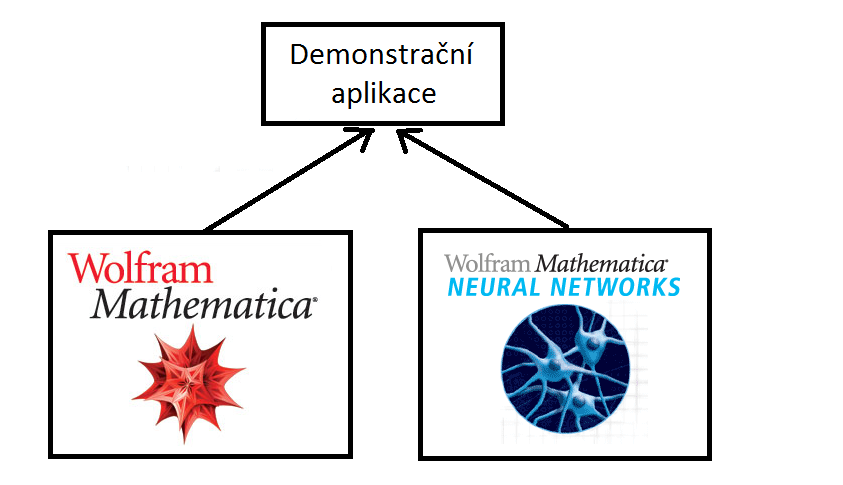
\includegraphics[width=10cm]{schema.png}
\end{figure}
\end{frame}

\begin{frame}{Struktura aplikace}
\begin{footnotesize}
\begin{table}[t]
\begin{tabular}{|c|l|l|}
\hline 
Kapitola & Název kapitoly & Soubor \\ \hline
1 & Úvod & 01-uvod.nb \\ \hline
2 & Algoritmy učení & 02-algoritmy-uceni.nb \\ \hline
3 & Křížová validace & 03-crossvalidation.nb \\ \hline
4 & Dopředná síť a umělá data sin(x) & 04-feedforward-sin.nb \\ \hline
5 & Dopředná síť a Iris data & 05-feedforward-iris.nb \\ \hline
6 & Přístupy k učení dopředné sítě & 06-feedforward-iris-2.nb \\ \hline
7 & Pokrytí dat jednoduchou RBF sítí & 07-rbf-neuron.nb \\ \hline
8 & Pokrytí dat RBF sítí & 08-rbf-neuron-2.nb \\ \hline
9 & Síť RBF a umělá data sin(x) & 09-rbf-sin.nb \\ \hline
10 & Síť RBF a Iris data & 10-rbf-iris.nb \\ \hline
11 & Přístupy k učení RBF sítě & 11-rbf-iris-2.nb \\ \hline
12 & Hopfieldova síť a umělé vzory & 12-hopfield.nb \\ \hline
13 & Shlukování dat sítí bez učitele & 13-som-clustering.nb \\ \hline
14 & Kohonenova síť a Iris data & 14-som-iris.nb \\ \hline
15 & LVQ a Iris data & 15-lvq-iris.nb \\ \hline
\end{tabular}
\label{tab:aplikace}
\end{table}
\end{footnotesize}
\end{frame}

\begin{frame}{Struktura souboru}
\begin{figure}
   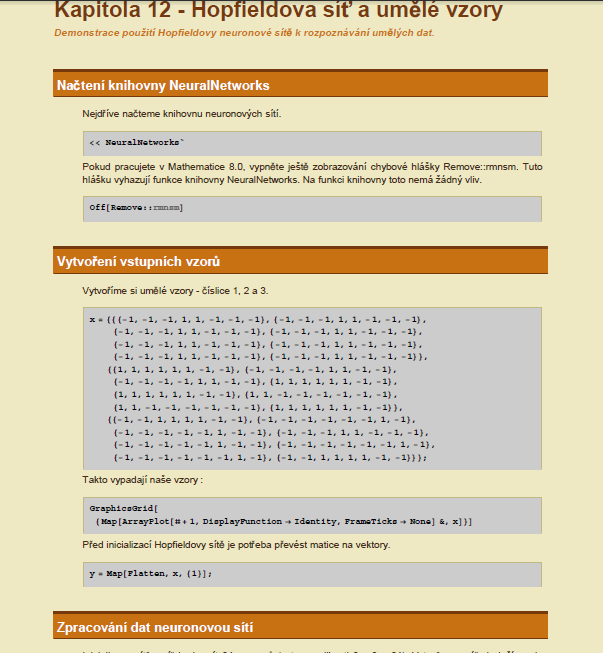
\includegraphics[width=6cm]{ukc1.png}
\end{figure}
\end{frame}

\begin{frame}{Dělení souborů podle obsahu}
\begin{itemize}
\item Soubory demonstrující principy neuronových sítí
\item Soubory demonstrující použití neuronových sítí
\item Soubory demonstrující vyhodnocení neuronových sítí
\end{itemize}
\end{frame}
\begin{frame}{Demonstrace principu neuronové sítě}
\begin{itemize}
\item Slouží k pochopení vnitřní funkcionality sítě a učicích algoritmů
\end{itemize} 
  \begin{columns}[T]
    \column{5cm}
      \begin{figure}
     
   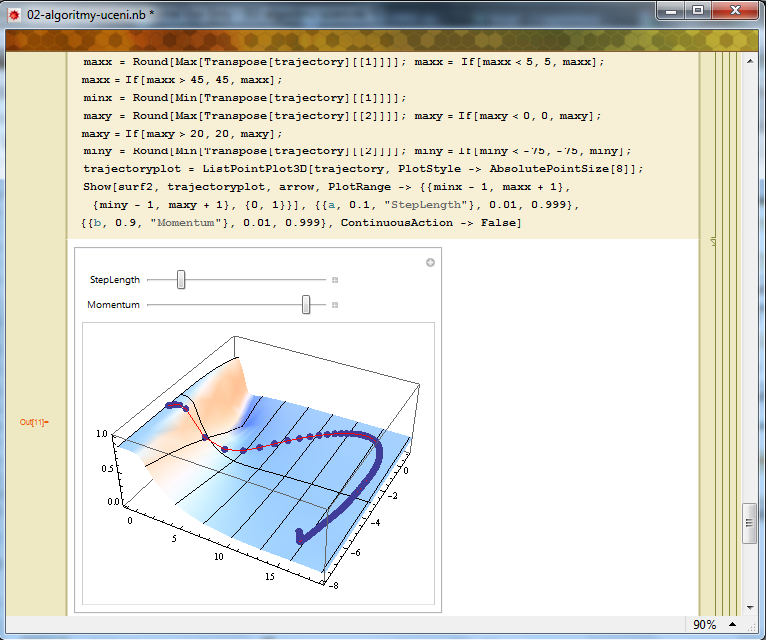
\includegraphics[width=5.5cm]{uk1.png}
    \caption{02-algoritmy-uceni.nb}
   
\end{figure}
    \column{5cm}
      \begin{figure}
   
   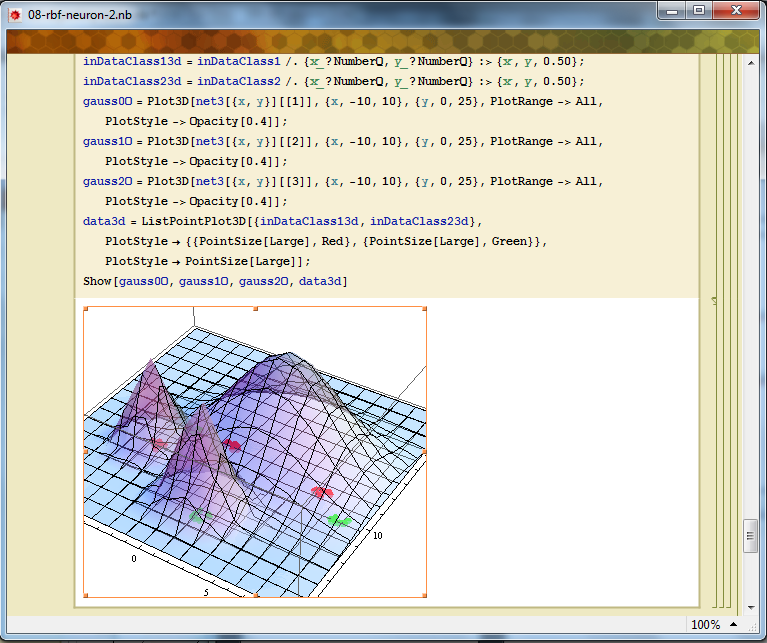
\includegraphics[width=5.5cm]{uk2.png}
      \caption{08-rbf-neuron-2.nb}
\end{figure}
  \end{columns}
\end{frame}


\begin{frame}{Demonstrace použití neuronové sítě}
\begin{itemize}
\item Demonstrují vytváření a jednoduchou práci s neuronovými sítěmi
\end{itemize} 
  \begin{columns}[T]
    \column{5cm}
      \begin{figure}
   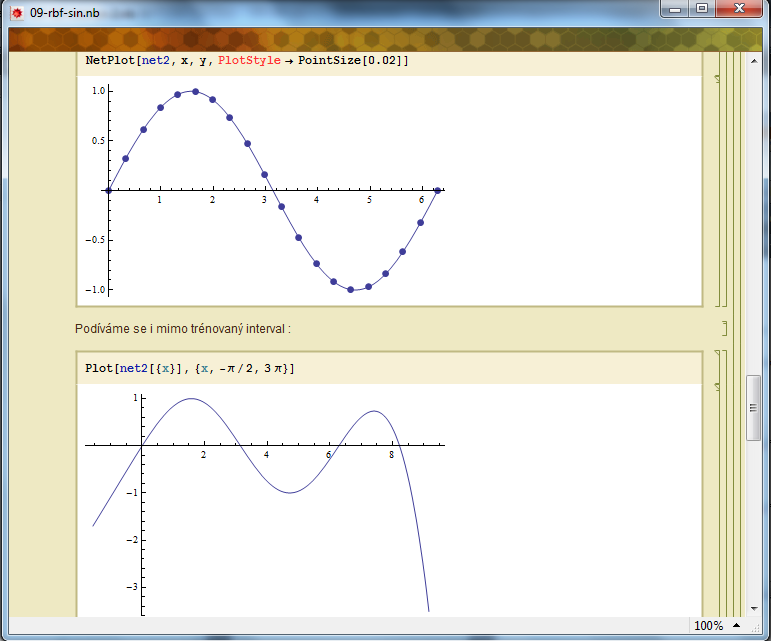
\includegraphics[width=5.5cm]{uk3.png}
   \caption{09-rbf-sin.nb}
\end{figure}
    \column{5cm}
      \begin{figure}
   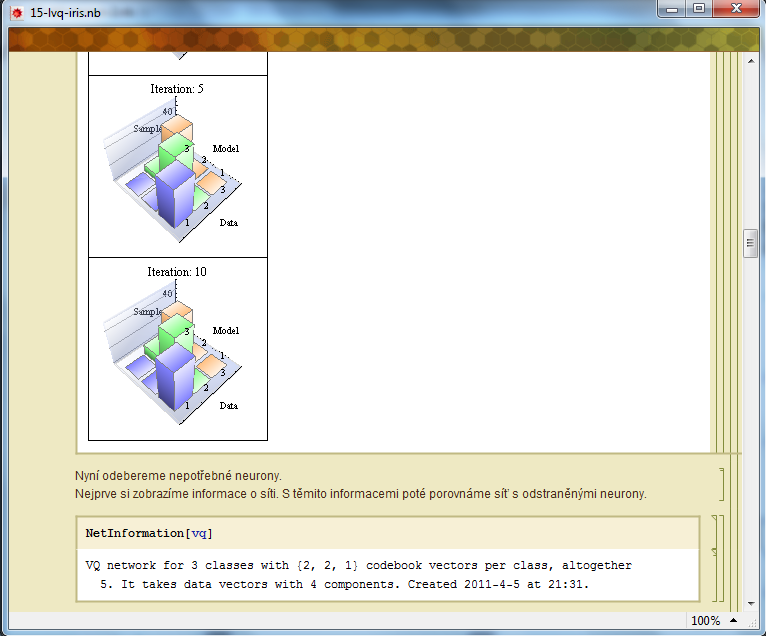
\includegraphics[width=5.5cm]{uk4.png}
   \caption{15-lvq-iris.nb}
\end{figure}
  \end{columns}
\end{frame}

\begin{frame}{Demonstrace vyhodnocení neuronové sítě}
\begin{itemize}
\item Ukazují jakými způsoby zhodnotit výstup sítě
\end{itemize} 
  \begin{columns}[T]
    \column{5cm}
      \begin{figure}
   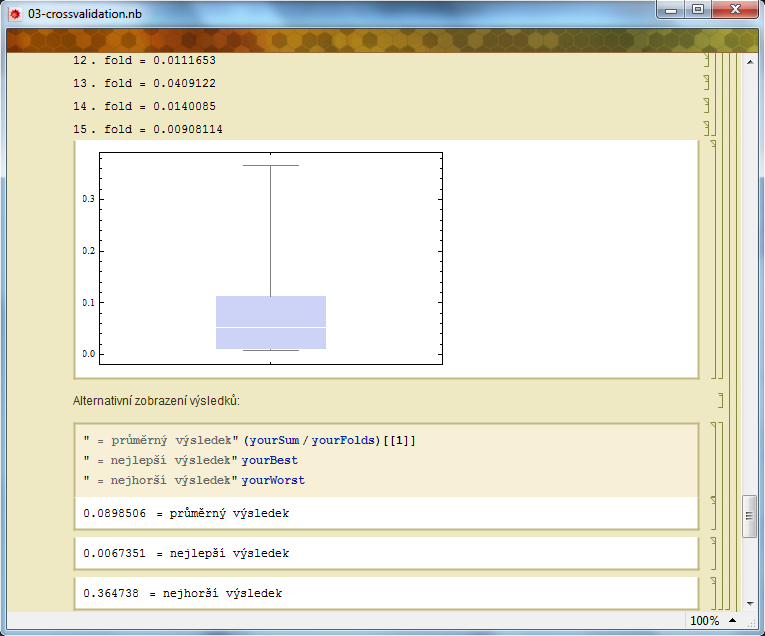
\includegraphics[width=5.5cm]{uk5.png}
   \caption{03-crossvalidation.nb}
\end{figure}
    \column{5cm}
      \begin{figure}
   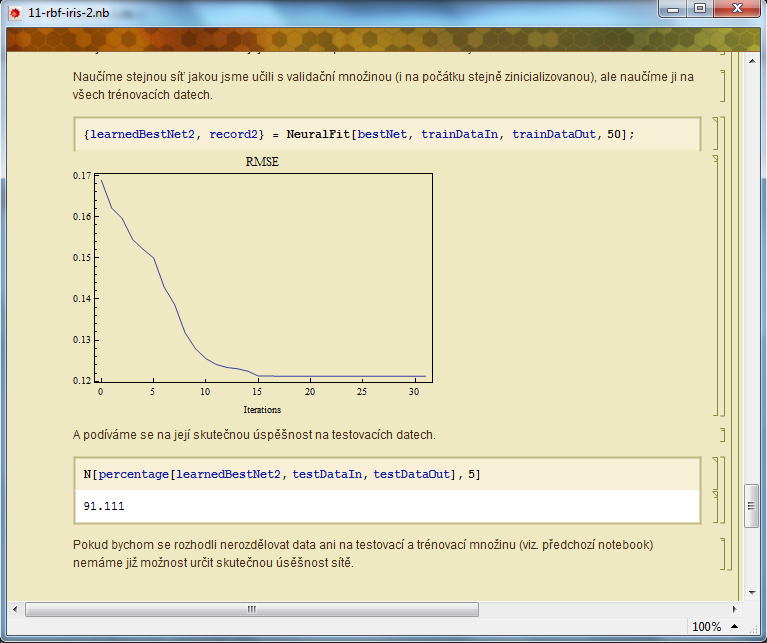
\includegraphics[width=5.5cm]{uk6.png}
   \caption{11-rbf-iris-2.nb}
\end{figure}
  \end{columns}
\end{frame}

\section{Teoretická část práce}
\begin{frame}{Teoretická část práce}
\begin{itemize}
\item Historický úvod do problematiky neuronových sítí
\item Popis neuronu a jeho fungování
\item Popis neuronových sítí včetně jejich algoritmů učení. Konkrétně jsou popsány:
\begin{itemize}
\item Dopředná síť
\item RBF síť
\item Hopfieldova síť
\item Samoorganizující mapa
\item LVQ síť
\end{itemize}
\item Popis křížové validace
\end{itemize}
\end{frame}

\begin{frame}{Výstup práce}
\begin{itemize}
\item Demonstrační aplikace - 15 interaktivních souborů
\item Doprovodný teoretický text
\item HTML stránka
\end{itemize}
\end{frame}

\begin{frame}{Zhodnocení práce}
\begin{itemize}
\item Výrazně jsem rozšířil Courseware k neuronovým sítím
\item Aplikace bude použita při výuce předmětu 36NAN
\item Její využití je možné i v dalších předmětech
\end{itemize}
\begin{itemize}
\item Seznámil jsem se s programováním v prostředí Mathematica
\item Výrazně si rozšířil znalosti v oblasti neuronových sítí
\item Naučil jsem se používat LaTeX
\end{itemize}
\end{frame}


\begin{frame}{Závěr}
\begin{center}
\begin{huge}
Děkuji za pozornost.
\end{huge}
\end{center}

\end{frame}
\end{document}